% Options for packages loaded elsewhere
\PassOptionsToPackage{unicode}{hyperref}
\PassOptionsToPackage{hyphens}{url}
%
\documentclass[
]{article}
\usepackage{amsmath,amssymb}
\usepackage{iftex}
\ifPDFTeX
  \usepackage[T1]{fontenc}
  \usepackage[utf8]{inputenc}
  \usepackage{textcomp} % provide euro and other symbols
\else % if luatex or xetex
  \usepackage{unicode-math} % this also loads fontspec
  \defaultfontfeatures{Scale=MatchLowercase}
  \defaultfontfeatures[\rmfamily]{Ligatures=TeX,Scale=1}
\fi
\usepackage{lmodern}
\ifPDFTeX\else
  % xetex/luatex font selection
\fi
% Use upquote if available, for straight quotes in verbatim environments
\IfFileExists{upquote.sty}{\usepackage{upquote}}{}
\IfFileExists{microtype.sty}{% use microtype if available
  \usepackage[]{microtype}
  \UseMicrotypeSet[protrusion]{basicmath} % disable protrusion for tt fonts
}{}
\makeatletter
\@ifundefined{KOMAClassName}{% if non-KOMA class
  \IfFileExists{parskip.sty}{%
    \usepackage{parskip}
  }{% else
    \setlength{\parindent}{0pt}
    \setlength{\parskip}{6pt plus 2pt minus 1pt}}
}{% if KOMA class
  \KOMAoptions{parskip=half}}
\makeatother
\usepackage{xcolor}
\usepackage[margin=1in]{geometry}
\usepackage{color}
\usepackage{fancyvrb}
\newcommand{\VerbBar}{|}
\newcommand{\VERB}{\Verb[commandchars=\\\{\}]}
\DefineVerbatimEnvironment{Highlighting}{Verbatim}{commandchars=\\\{\}}
% Add ',fontsize=\small' for more characters per line
\usepackage{framed}
\definecolor{shadecolor}{RGB}{248,248,248}
\newenvironment{Shaded}{\begin{snugshade}}{\end{snugshade}}
\newcommand{\AlertTok}[1]{\textcolor[rgb]{0.94,0.16,0.16}{#1}}
\newcommand{\AnnotationTok}[1]{\textcolor[rgb]{0.56,0.35,0.01}{\textbf{\textit{#1}}}}
\newcommand{\AttributeTok}[1]{\textcolor[rgb]{0.13,0.29,0.53}{#1}}
\newcommand{\BaseNTok}[1]{\textcolor[rgb]{0.00,0.00,0.81}{#1}}
\newcommand{\BuiltInTok}[1]{#1}
\newcommand{\CharTok}[1]{\textcolor[rgb]{0.31,0.60,0.02}{#1}}
\newcommand{\CommentTok}[1]{\textcolor[rgb]{0.56,0.35,0.01}{\textit{#1}}}
\newcommand{\CommentVarTok}[1]{\textcolor[rgb]{0.56,0.35,0.01}{\textbf{\textit{#1}}}}
\newcommand{\ConstantTok}[1]{\textcolor[rgb]{0.56,0.35,0.01}{#1}}
\newcommand{\ControlFlowTok}[1]{\textcolor[rgb]{0.13,0.29,0.53}{\textbf{#1}}}
\newcommand{\DataTypeTok}[1]{\textcolor[rgb]{0.13,0.29,0.53}{#1}}
\newcommand{\DecValTok}[1]{\textcolor[rgb]{0.00,0.00,0.81}{#1}}
\newcommand{\DocumentationTok}[1]{\textcolor[rgb]{0.56,0.35,0.01}{\textbf{\textit{#1}}}}
\newcommand{\ErrorTok}[1]{\textcolor[rgb]{0.64,0.00,0.00}{\textbf{#1}}}
\newcommand{\ExtensionTok}[1]{#1}
\newcommand{\FloatTok}[1]{\textcolor[rgb]{0.00,0.00,0.81}{#1}}
\newcommand{\FunctionTok}[1]{\textcolor[rgb]{0.13,0.29,0.53}{\textbf{#1}}}
\newcommand{\ImportTok}[1]{#1}
\newcommand{\InformationTok}[1]{\textcolor[rgb]{0.56,0.35,0.01}{\textbf{\textit{#1}}}}
\newcommand{\KeywordTok}[1]{\textcolor[rgb]{0.13,0.29,0.53}{\textbf{#1}}}
\newcommand{\NormalTok}[1]{#1}
\newcommand{\OperatorTok}[1]{\textcolor[rgb]{0.81,0.36,0.00}{\textbf{#1}}}
\newcommand{\OtherTok}[1]{\textcolor[rgb]{0.56,0.35,0.01}{#1}}
\newcommand{\PreprocessorTok}[1]{\textcolor[rgb]{0.56,0.35,0.01}{\textit{#1}}}
\newcommand{\RegionMarkerTok}[1]{#1}
\newcommand{\SpecialCharTok}[1]{\textcolor[rgb]{0.81,0.36,0.00}{\textbf{#1}}}
\newcommand{\SpecialStringTok}[1]{\textcolor[rgb]{0.31,0.60,0.02}{#1}}
\newcommand{\StringTok}[1]{\textcolor[rgb]{0.31,0.60,0.02}{#1}}
\newcommand{\VariableTok}[1]{\textcolor[rgb]{0.00,0.00,0.00}{#1}}
\newcommand{\VerbatimStringTok}[1]{\textcolor[rgb]{0.31,0.60,0.02}{#1}}
\newcommand{\WarningTok}[1]{\textcolor[rgb]{0.56,0.35,0.01}{\textbf{\textit{#1}}}}
\usepackage{graphicx}
\makeatletter
\def\maxwidth{\ifdim\Gin@nat@width>\linewidth\linewidth\else\Gin@nat@width\fi}
\def\maxheight{\ifdim\Gin@nat@height>\textheight\textheight\else\Gin@nat@height\fi}
\makeatother
% Scale images if necessary, so that they will not overflow the page
% margins by default, and it is still possible to overwrite the defaults
% using explicit options in \includegraphics[width, height, ...]{}
\setkeys{Gin}{width=\maxwidth,height=\maxheight,keepaspectratio}
% Set default figure placement to htbp
\makeatletter
\def\fps@figure{htbp}
\makeatother
\setlength{\emergencystretch}{3em} % prevent overfull lines
\providecommand{\tightlist}{%
  \setlength{\itemsep}{0pt}\setlength{\parskip}{0pt}}
\setcounter{secnumdepth}{5}
% Load necessary packages
\usepackage{amsmath}    % For advanced math typesetting
\usepackage{graphicx}   % For including images
\usepackage{hyperref}   % For hyperlinks
\usepackage{geometry}   % For setting page dimensions
\usepackage{fancyhdr}   % For custom headers and footers
\usepackage{setspace}   % For setting line spacing

% Set page dimensions
\geometry{
  a4paper,
  left=25mm,
  right=25mm,
  top=25mm,
  bottom=25mm
}

% Custom header and footer
\pagestyle{fancy}
\fancyhf{}
\fancyhead[L]{\leftmark}
\fancyhead[R]{\thepage}

% Custom commands
\newcommand{\HRule}{\rule{\linewidth}{0.5mm}}

% Set line spacing
\setstretch{1.5}

% Additional settings
\hypersetup{
  colorlinks=true,
  linkcolor=blue,
  filecolor=magenta,
  urlcolor=cyan,
  pdftitle={Your Document Title},
  pdfpagemode=FullScreen,
}
\ifLuaTeX
  \usepackage{selnolig}  % disable illegal ligatures
\fi
\IfFileExists{bookmark.sty}{\usepackage{bookmark}}{\usepackage{hyperref}}
\IfFileExists{xurl.sty}{\usepackage{xurl}}{} % add URL line breaks if available
\urlstyle{same}
\hypersetup{
  pdftitle={C91AR \textbar{} Advanced Statistics using R},
  pdfauthor={Dr Pete McKenna},
  hidelinks,
  pdfcreator={LaTeX via pandoc}}

\title{C91AR \textbar{} Advanced Statistics using R}
\usepackage{etoolbox}
\makeatletter
\providecommand{\subtitle}[1]{% add subtitle to \maketitle
  \apptocmd{\@title}{\par {\large #1 \par}}{}{}
}
\makeatother
\subtitle{Lecture 6: Data Simulation for Correlation in R}
\author{Dr Pete McKenna}
\date{2025-02-28}

\begin{document}
\maketitle

{
\setcounter{tocdepth}{2}
\tableofcontents
}
\hypertarget{todays-packages}{%
\section{Todays packages}\label{todays-packages}}

\begin{Shaded}
\begin{Highlighting}[]
\CommentTok{\# load packages}
\NormalTok{pacman}\SpecialCharTok{::}\FunctionTok{p\_load}\NormalTok{(tidyverse,}
\NormalTok{               corrr,}
\NormalTok{               psych,}
\NormalTok{               tidyplots)}
\end{Highlighting}
\end{Shaded}

\hypertarget{whats-the-deal-with-data-simulation}{%
\section{What's the deal with data
simulation?}\label{whats-the-deal-with-data-simulation}}

\begin{itemize}
\tightlist
\item
  Simulating data is a really useful skill for research and teaching.
\item
  For research, it can help you to plan and prepare analysis scripts
  (e.g., for pre-registration), instead of waiting until data collection
  is complete.

  \begin{itemize}
  \tightlist
  \item
    This in turn can help you select the correct statistical test.
  \end{itemize}
\item
  For teaching, you can create topic-relevant datasets for specific
  courses.
\item
  More generally, creating and working with simulated data helps to
  develop your understanding of statistical concepts.
\end{itemize}

\hypertarget{ok-so-what-is-todays-session-going-to-cover}{%
\section{OK, so what is today's session going to
cover?}\label{ok-so-what-is-todays-session-going-to-cover}}

\begin{itemize}
\tightlist
\item
  The formula for correlation
\item
  The related R code for simulating bivariate (i.e., includes 2
  variables) data
\item
  How to plot simulated data
\end{itemize}

\hypertarget{simulating-univariate-data}{%
\section{Simulating Univariate data}\label{simulating-univariate-data}}

\begin{itemize}
\tightlist
\item
  Data along a normal distribution can be simulated using the
  \texttt{rnorm} function, like so:
\end{itemize}

\begin{Shaded}
\begin{Highlighting}[]
\FunctionTok{set.seed}\NormalTok{(}\DecValTok{385}\NormalTok{) }\CommentTok{\# seed a random number for reproducibility}

\CommentTok{\# Say we wanted to simulate response time to a cogntive test}
\CommentTok{\# where the mean = 1000, the SD = 50, from 150 participants}

\NormalTok{rt\_sim }\OtherTok{\textless{}{-}} 
  \FunctionTok{tibble}\NormalTok{(                         }\CommentTok{\# create data table object}
  \AttributeTok{control\_rt =} \FunctionTok{rnorm}\NormalTok{(}\AttributeTok{mean =} \DecValTok{1000}\NormalTok{, }\CommentTok{\# state the mean }
                     \AttributeTok{sd =} \DecValTok{500}\NormalTok{,    }\CommentTok{\# provide the sd}
                     \AttributeTok{n =} \DecValTok{150}\NormalTok{))    }\CommentTok{\# supply the sample size}
\end{Highlighting}
\end{Shaded}

\hypertarget{examine-the-data}{%
\section{Examine the data}\label{examine-the-data}}

\begin{Shaded}
\begin{Highlighting}[]
\FunctionTok{headTail}\NormalTok{(rt\_sim)}
\end{Highlighting}
\end{Shaded}

\begin{verbatim}
##   control_rt
## 1    1443.73
## 2    1568.94
## 3     808.48
## 4     699.91
## 5        ...
## 6     428.12
## 7     773.09
## 8     663.01
## 9     859.12
\end{verbatim}

\begin{center}\rule{0.5\linewidth}{0.5pt}\end{center}

\begin{itemize}
\tightlist
\item
  Here's our data plotted in a histogram.
\end{itemize}

\begin{Shaded}
\begin{Highlighting}[]
\CommentTok{\# generate the histogram with ggplot2}
\FunctionTok{ggplot}\NormalTok{(}\AttributeTok{data =}\NormalTok{ rt\_sim,                   }\CommentTok{\# specify data source}
       \AttributeTok{mapping =} \FunctionTok{aes}\NormalTok{(}\AttributeTok{x =}\NormalTok{ control\_rt)) }\SpecialCharTok{+} \CommentTok{\# specify x and y mapping}
  \FunctionTok{geom\_histogram}\NormalTok{() }\SpecialCharTok{+}                    \CommentTok{\# add histogram layer}
  \FunctionTok{labs}\NormalTok{(}\AttributeTok{x =} \StringTok{"}\SpecialCharTok{\textbackslash{}n}\StringTok{Response time (ms)"}\NormalTok{)      }\CommentTok{\# supply axis labels}
\end{Highlighting}
\end{Shaded}

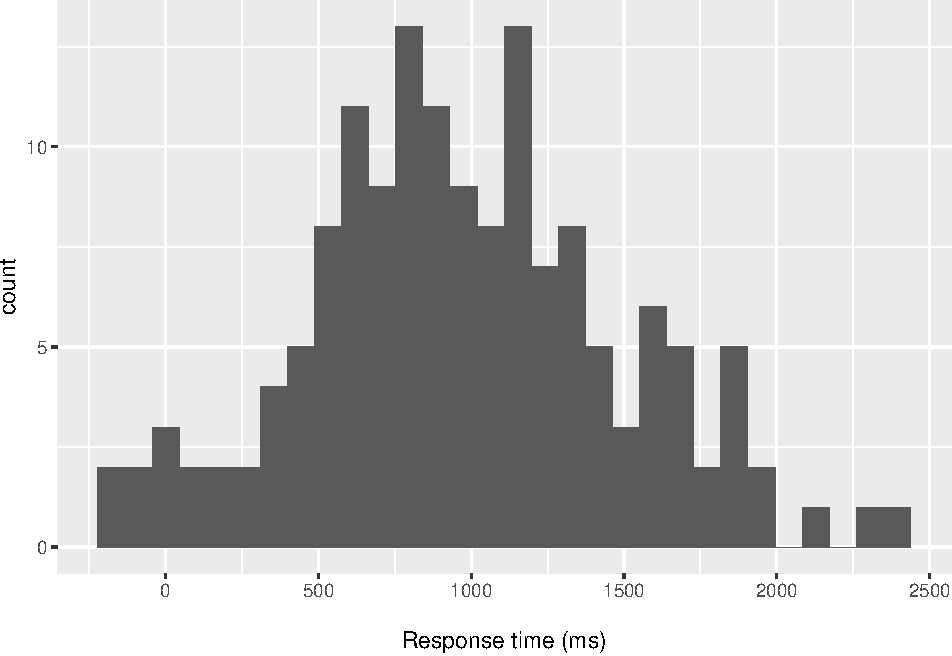
\includegraphics{L6_Correlation_and_regresion_simulation_pdf_files/figure-latex/rnorm plot-1.pdf}

\hypertarget{how-not-to-simulate-bivariate-data}{%
\section{\texorpdfstring{How \textbf{NOT} To Simulate Bivariate
data}{How NOT To Simulate Bivariate data}}\label{how-not-to-simulate-bivariate-data}}

\begin{itemize}
\tightlist
\item
  However, to simulate the distribution of two related variables you
  can't just run \texttt{rnorm} twice as you will end up with two
  variables that are unrelated, with a correlation of (near) zero.
\end{itemize}

\begin{Shaded}
\begin{Highlighting}[]
\CommentTok{\# simulate two separate datasets}
\NormalTok{data }\OtherTok{\textless{}{-}} 
  \FunctionTok{tibble}\NormalTok{(}
  \AttributeTok{control\_rt =} \FunctionTok{rnorm}\NormalTok{(}\AttributeTok{mean =} \DecValTok{1000}\NormalTok{, }
                     \AttributeTok{sd =} \DecValTok{500}\NormalTok{,}
                     \AttributeTok{n =} \DecValTok{150}\NormalTok{),}
  \AttributeTok{treatment\_rt =} \FunctionTok{rnorm}\NormalTok{(}\AttributeTok{mean =} \DecValTok{1200}\NormalTok{, }
                       \AttributeTok{sd =} \DecValTok{700}\NormalTok{,}
                       \AttributeTok{n =} \DecValTok{150}\NormalTok{))}

\CommentTok{\# run a correlation}
\FunctionTok{cor}\NormalTok{(data}\SpecialCharTok{$}\NormalTok{control\_rt,   }\CommentTok{\# Pearson is the default}
\NormalTok{    data}\SpecialCharTok{$}\NormalTok{treatment\_rt)}
\end{Highlighting}
\end{Shaded}

\begin{verbatim}
## [1] -0.0373358
\end{verbatim}

\hypertarget{our-first-attempt-at-simulating-multivariate-data}{%
\section{Our first attempt at simulating multivariate
data}\label{our-first-attempt-at-simulating-multivariate-data}}

\begin{itemize}
\tightlist
\item
  Let's start by simulating some data representing hypothetical humans
  and their height and weight.
\item
  We know these things are correlated.
\item
  What we need to be able to simulate are the \textbf{means},
  \textbf{standard deviations}, and the \textbf{correlations between
  these two variables}.
\item
  I'm using a dataset of heights and weights - link on final slide.
\end{itemize}

\begin{center}\rule{0.5\linewidth}{0.5pt}\end{center}

\begin{Shaded}
\begin{Highlighting}[]
\CommentTok{\# read in the data}
\CommentTok{\# make sure you include the full file name and type (e.g., .csv) in the quotes}
\NormalTok{handw }\OtherTok{\textless{}{-}} 
  \FunctionTok{read\_csv}\NormalTok{(}\StringTok{"data\_raw/heights\_and\_weights.csv"}\NormalTok{, }
           \AttributeTok{col\_types =} \StringTok{"dd"}\NormalTok{)                }\CommentTok{\# specify that both cols are \textasciigrave{}double\textasciigrave{} type}


\CommentTok{\# peek into heights and weights dataset}
\FunctionTok{glimpse}\NormalTok{(handw)}
\end{Highlighting}
\end{Shaded}

\begin{verbatim}
## Rows: 475
## Columns: 2
## $ height_in  <dbl> 63, 67, 71, 71, 56, 67, 65, 74, 64, 62, 60, 47, 38, 67, 67,~
## $ weight_lbs <dbl> 130, 169, 178, 225, 98, 204, 145, 180, 150, 136, 110, 80, 3~
\end{verbatim}

\hypertarget{scatter-plot-the-heights-and-weights-data}{%
\section{Scatter plot the heights and weights
data}\label{scatter-plot-the-heights-and-weights-data}}

\begin{Shaded}
\begin{Highlighting}[]
\CommentTok{\# generate the scatter plot with ggplot2}
\FunctionTok{ggplot}\NormalTok{(}\AttributeTok{data =}\NormalTok{ handw,                                    }\CommentTok{\# specify data source}
       \AttributeTok{mapping =} \FunctionTok{aes}\NormalTok{(}\AttributeTok{x =}\NormalTok{ height\_in, }\AttributeTok{y =}\NormalTok{ weight\_lbs)) }\SpecialCharTok{+}  \CommentTok{\# specify x and y axis}
  \FunctionTok{geom\_point}\NormalTok{(}\AttributeTok{alpha =}\NormalTok{ .}\DecValTok{6}\NormalTok{) }\SpecialCharTok{+}                              \CommentTok{\# modify transparency of points}
  \FunctionTok{labs}\NormalTok{(}\AttributeTok{x =} \StringTok{"}\SpecialCharTok{\textbackslash{}n}\StringTok{Height (inches)"}\NormalTok{,                         }\CommentTok{\# supply axis label names}
       \AttributeTok{y =} \StringTok{"Weight (pounds)}\SpecialCharTok{\textbackslash{}n}\StringTok{"}\NormalTok{)}
\end{Highlighting}
\end{Shaded}

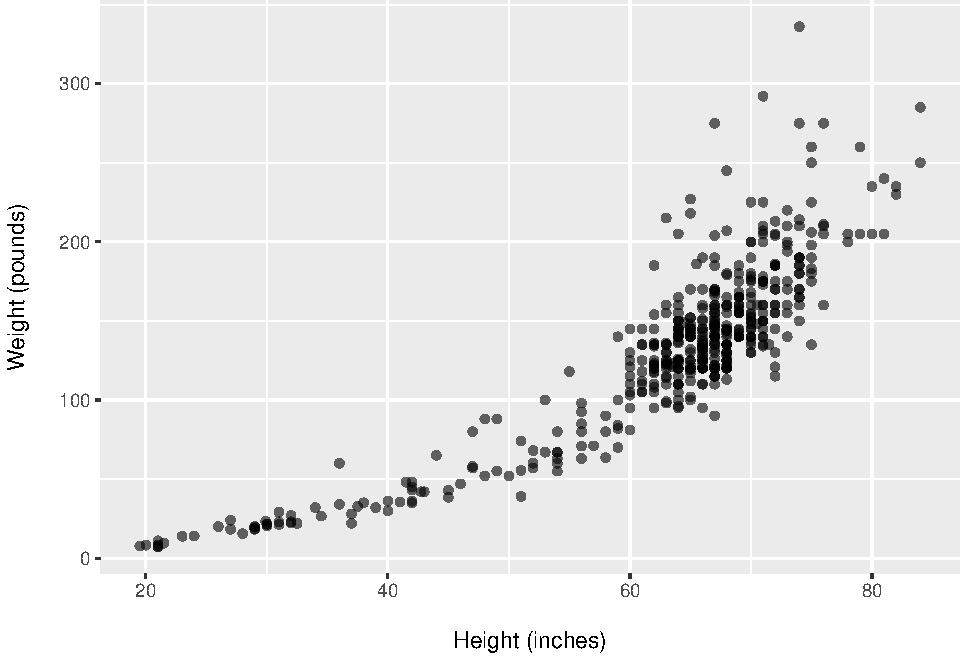
\includegraphics{L6_Correlation_and_regresion_simulation_pdf_files/figure-latex/plot handw-1.pdf}

\begin{itemize}
\tightlist
\item
  It is evident from the scatter plot of the distribution that the
  relationship between heights and weights is not quite linear, so let's
  log transform the variables.
\end{itemize}

\hypertarget{scatter-plot-of-the-log-of-handw-data}{%
\section{\texorpdfstring{Scatter plot of the log of \texttt{handw}
data}{Scatter plot of the log of handw data}}\label{scatter-plot-of-the-log-of-handw-data}}

\begin{Shaded}
\begin{Highlighting}[]
\CommentTok{\# add log transformed vectors to dataset}
\NormalTok{handw\_log }\OtherTok{\textless{}{-}}
\NormalTok{  handw }\SpecialCharTok{|\textgreater{}}
  \FunctionTok{mutate}\NormalTok{(}\AttributeTok{hlog =} \FunctionTok{log}\NormalTok{(height\_in),  }\CommentTok{\# create new variable \textasciigrave{}hlog\textasciigrave{} which is the log of height\_in}
         \AttributeTok{wlog =} \FunctionTok{log}\NormalTok{(weight\_lbs)) }\CommentTok{\# create new variable \textasciigrave{}wlog\textasciigrave{} which is the log of weight\_lbs}

\CommentTok{\# generate a scatter plot of the log data}
\FunctionTok{ggplot}\NormalTok{(}\AttributeTok{data =}\NormalTok{ handw\_log,                      }\CommentTok{\# don\textquotesingle{}t forget to enter the new dataset              }
       \AttributeTok{mapping =} \FunctionTok{aes}\NormalTok{(}\AttributeTok{x =}\NormalTok{ hlog, }\AttributeTok{y =}\NormalTok{ wlog)) }\SpecialCharTok{+}  
  \FunctionTok{geom\_point}\NormalTok{(}\AttributeTok{alpha =}\NormalTok{ .}\DecValTok{6}\NormalTok{) }\SpecialCharTok{+}                              
  \FunctionTok{labs}\NormalTok{(}\AttributeTok{x =} \StringTok{"}\SpecialCharTok{\textbackslash{}n}\StringTok{Log(Height)"}\NormalTok{,                           }
       \AttributeTok{y =} \StringTok{"log(Weight)}\SpecialCharTok{\textbackslash{}n}\StringTok{"}\NormalTok{)}
\end{Highlighting}
\end{Shaded}

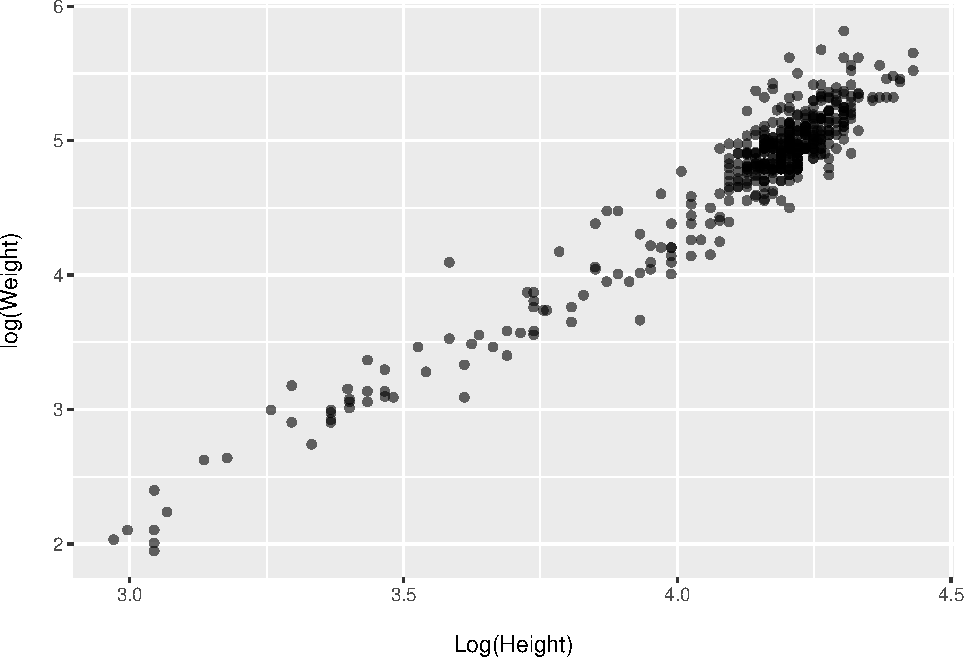
\includegraphics{L6_Correlation_and_regresion_simulation_pdf_files/figure-latex/log transform the handw data-1.pdf}

\hypertarget{using-the-massmvrnorm-command}{%
\section{\texorpdfstring{Using the \texttt{MASS::mvrnorm}
command}{Using the MASS::mvrnorm command}}\label{using-the-massmvrnorm-command}}

\begin{itemize}
\tightlist
\item
  The \texttt{MASS} package provides a function \texttt{mvronrm} which
  stands for multivariate + \texttt{rnorm}.
\item
  \texttt{MASS} is a large package in R, so for efficiency let's only
  load the required components by using the argument
  \texttt{MASS::mvrnorm} instead of \texttt{library("MASS")}.
\item
  This is also a handy way to proceed as there are some annoying package
  conflicts between \texttt{dplyr} and \texttt{MASS} that we want to
  avoid.
\end{itemize}

\hypertarget{massmvrnorm-arguments}{%
\section{\texorpdfstring{\texttt{MASS::mvrnorm}
arguments}{MASS::mvrnorm arguments}}\label{massmvrnorm-arguments}}

\begin{itemize}
\tightlist
\item
  The three arguments to take note of are:

  \begin{itemize}
  \tightlist
  \item
    \texttt{n} = number of samples required
  \item
    \texttt{mu} = a vector giving the means of the variables
  \item
    \texttt{Sigma} = a positive-definite symmetric matrix specifying the
    covariance of the variables
  \end{itemize}
\item
  \emph{Positive-Definite Symmetric Matrix}

  \begin{itemize}
  \tightlist
  \item
    A covariance matrix (also known as the variance-covariance matrix)
    specifying the variances of the individual variables and their
    inter-relationships.
  \item
    It is essentially a multi-dimensional version of standard deviation.
  \end{itemize}
\end{itemize}

\hypertarget{out-of-interest-what-about-the-relationship-between-2-variables}{%
\subsection{Out of interest, what about the relationship between 2+
variables?}\label{out-of-interest-what-about-the-relationship-between-2-variables}}

For a multivariate distribution with more than two variables you need

\begin{itemize}
\tightlist
\item
  The means for all of the variables.
\item
  Their standard deviations.
\item
  All possible pairwise correlations between the variables.
\end{itemize}

\hypertarget{matrix-calculations-for-the-sigma-argument}{%
\section{\texorpdfstring{Matrix Calculations for the \emph{Sigma}
argument}{Matrix Calculations for the Sigma argument}}\label{matrix-calculations-for-the-sigma-argument}}

A covariance matrix can be calculated using the following formula:

\[
\sum = \begin{pmatrix}\sigma_x^2 & \rho_{xy}\sigma_x\sigma_y \\ \rho_{yx}\sigma_y\sigma_x & \sigma_y^2 \end{pmatrix}
\]

\begin{itemize}
\tightlist
\item
  \(\sigma_x^2\) = squared SD for \(x\).
\item
  \(\sigma_y^2\) = squared SD \(y\).
\item
  \(\rho_{xy}\sigma_x\sigma_y\) = the co-variances (i.e., the
  correlation multiplied by the two standard deviations, shown in the
  off-diagonal.
\item
  It is worth saying here that the \textbf{covariance is just the
  correlation times the product of the two standard deviations.}
\end{itemize}

\hypertarget{gathering-the-statistics}{%
\section{Gathering the statistics}\label{gathering-the-statistics}}

\begin{itemize}
\tightlist
\item
  Let's start by gathering the statistics we need to simulate the data
  using \texttt{MASS::mvrnorm}.
\item
  Remember, we need the

  \begin{itemize}
  \tightlist
  \item
    \texttt{mean}
  \item
    \texttt{sd}
  \item
    \texttt{Sigma}
  \end{itemize}
\item
  We will continue with the log of the data, as the relationship is more
  linear.
\end{itemize}

\begin{center}\rule{0.5\linewidth}{0.5pt}\end{center}

\begin{Shaded}
\begin{Highlighting}[]
\CommentTok{\# calculate means and sd}
\NormalTok{handw\_log }\SpecialCharTok{|\textgreater{}}
  \FunctionTok{summarise}\NormalTok{(}\AttributeTok{mean\_h =} \FunctionTok{mean}\NormalTok{(hlog),}
            \AttributeTok{sd\_h =} \FunctionTok{sd}\NormalTok{(hlog),}
            \AttributeTok{mean\_w =} \FunctionTok{mean}\NormalTok{(wlog),}
            \AttributeTok{sd\_w =} \FunctionTok{sd}\NormalTok{(wlog)) }\SpecialCharTok{|\textgreater{}}
  \FunctionTok{mutate\_if}\NormalTok{(is.numeric, round, }\AttributeTok{digits =} \DecValTok{2}\NormalTok{) }\CommentTok{\# round to 2 decimal places}
\end{Highlighting}
\end{Shaded}

\begin{verbatim}
## # A tibble: 1 x 4
##   mean_h  sd_h mean_w  sd_w
##    <dbl> <dbl>  <dbl> <dbl>
## 1   4.11  0.26   4.74  0.65
\end{verbatim}

\begin{Shaded}
\begin{Highlighting}[]
\CommentTok{\# calculate correlation}
\FunctionTok{cor}\NormalTok{(handw\_log}\SpecialCharTok{$}\NormalTok{hlog, handw\_log}\SpecialCharTok{$}\NormalTok{wlog)}
\end{Highlighting}
\end{Shaded}

\begin{verbatim}
## [1] 0.9615714
\end{verbatim}

\hypertarget{calculation-output}{%
\section{Calculation output}\label{calculation-output}}

\begin{itemize}
\tightlist
\item
  \(\bar{x} = 4.11, \sigma_x = 0.26\) (mean and SD of log height)
\item
  \(\bar{y} = 4.74, \sigma_y = 0.65\) (mean and SD of log weight)
\item
  \(\rho_{xy} = 0.96\) (correlation between the two)
\end{itemize}

\hypertarget{calculating-sigma-for-massmvrnorm}{%
\section{\texorpdfstring{Calculating \emph{Sigma} for
\texttt{MASS:mvrnorm}}{Calculating Sigma for MASS:mvrnorm}}\label{calculating-sigma-for-massmvrnorm}}

\begin{itemize}
\tightlist
\item
  We now have all of the information we need to simulate the height and
  weight of, let's say 500 humans.
\item
  One last piece in the puzzle is to create the covariance matrix to
  supply to the \texttt{Sigma} argument.
\item
  Let's plug in the output values we calculated previously into the
  covariance matrix formula.
\end{itemize}

\hypertarget{enter-values-into-the-formula}{%
\section{Enter values into the
formula}\label{enter-values-into-the-formula}}

\[
\sum = \begin{pmatrix}\sigma_x^2 & \rho_{xy}\sigma_x\sigma_y \\ \rho_{yx}\sigma_y\sigma_x & \sigma_y^2 \end{pmatrix}
\]

\begin{itemize}
\tightlist
\item
  So plugging in the values we got above, our covariance matrix should
  be
\end{itemize}

\[\sum = \begin{pmatrix}
.26^2 & (.96)(.26)(.65) \\
(.96)(.65)(.26) & .65^2
\end{pmatrix} = \begin{pmatrix}
.067 & .162\\
.162 & .423
\end{pmatrix}\]

\hypertarget{create-covariance-matrix-for-the-massmvrnorm-argument-in-r}{%
\section{\texorpdfstring{Create covariance matrix for the
\texttt{MASS::mvrnorm} argument in
R}{Create covariance matrix for the MASS::mvrnorm argument in R}}\label{create-covariance-matrix-for-the-massmvrnorm-argument-in-r}}

\begin{Shaded}
\begin{Highlighting}[]
\CommentTok{\# define and store covariances}
\NormalTok{my\_cov }\OtherTok{\textless{}{-}} 
\NormalTok{  .}\DecValTok{96} \SpecialCharTok{*}\NormalTok{ .}\DecValTok{26} \SpecialCharTok{*}\NormalTok{ .}\DecValTok{65} \CommentTok{\# log of correlation times hlog\_sd times wlog\_sd}

\CommentTok{\# use the matrix function to define our sigma}
\NormalTok{my\_sigma }\OtherTok{\textless{}{-}}
  \FunctionTok{matrix}\NormalTok{(}\FunctionTok{c}\NormalTok{(.}\DecValTok{26}\SpecialCharTok{\^{}}\DecValTok{2}\NormalTok{, my\_cov, }
\NormalTok{           my\_cov, .}\DecValTok{65}\SpecialCharTok{\^{}}\DecValTok{2}\NormalTok{), }
         \AttributeTok{ncol =} \DecValTok{2}\NormalTok{)}

\NormalTok{my\_sigma          }\CommentTok{\# print the matrix}
\end{Highlighting}
\end{Shaded}

\begin{verbatim}
##         [,1]    [,2]
## [1,] 0.06760 0.16224
## [2,] 0.16224 0.42250
\end{verbatim}

\hypertarget{some-notes-about-the-matrix-function}{%
\subsection{\texorpdfstring{Some notes about the \texttt{matrix}
function}{Some notes about the matrix function}}\label{some-notes-about-the-matrix-function}}

\begin{itemize}
\tightlist
\item
  The first argument is a vector of values, which we created using
  \texttt{c()}.
\item
  The \texttt{ncol} argument specifies how many columns the matrix
  should have.
\item
  \texttt{matrix} fills the elements of the matrix by column by column,
  rather than row by row.
\item
  You can change this behaviour if desired by changing the byrow
  argument to \texttt{byrow\ =\ TRUE}.
\end{itemize}

\hypertarget{simulate-data}{%
\section{Simulate data}\label{simulate-data}}

OK, so now we have \texttt{my\_sigma} we're ready to use
\texttt{MASS::mvrnorm}. Let's test it by creating 6 synthetic humans.

\begin{Shaded}
\begin{Highlighting}[]
\CommentTok{\# pass the names vector c(height = 4.11, weight = 4.74)}
\CommentTok{\# for mu gives us column names in the output}
\NormalTok{log\_ht\_wt }\OtherTok{\textless{}{-}}
\NormalTok{  MASS}\SpecialCharTok{::}\FunctionTok{mvrnorm}\NormalTok{(}\AttributeTok{n =} \DecValTok{6}\NormalTok{,                 }\CommentTok{\# our 6 synthetic humans }
                \AttributeTok{mu =} \FunctionTok{c}\NormalTok{(}\AttributeTok{height =} \FloatTok{4.11}\NormalTok{,  }\CommentTok{\# log mean of height }
                       \AttributeTok{weight =} \FloatTok{4.74}\NormalTok{), }\CommentTok{\# log mean of weight}
                \AttributeTok{Sigma =}\NormalTok{ my\_sigma)      }\CommentTok{\# our positive{-}definitive matrix}

\CommentTok{\# view the output}
\NormalTok{log\_ht\_wt}
\end{Highlighting}
\end{Shaded}

\begin{verbatim}
##        height   weight
## [1,] 4.046250 4.964822
## [2,] 3.946070 4.613247
## [3,] 4.582814 5.702836
## [4,] 4.520118 5.680369
## [5,] 4.134257 4.573500
## [6,] 4.427730 5.442189
\end{verbatim}

\begin{center}\rule{0.5\linewidth}{0.5pt}\end{center}

\begin{itemize}
\tightlist
\item
  \texttt{MASS::mvrnorm} returns a matrix with a row for each simulated
  human, with the first column representing the log height and the
  second representing the log weight.
\item
  But the log heights and weights are not very useful to us, so let's
  transform them back using the \texttt{exp()}, which is the inverse of
  \texttt{log()} transform.
\end{itemize}

\begin{Shaded}
\begin{Highlighting}[]
\FunctionTok{exp}\NormalTok{(log\_ht\_wt)}
\end{Highlighting}
\end{Shaded}

\begin{verbatim}
##        height   weight
## [1,] 57.18263 143.2831
## [2,] 51.73166 100.8109
## [3,] 97.78919 299.7163
## [4,] 91.84645 293.0574
## [5,] 62.44320  96.8826
## [6,] 83.74115 230.9473
\end{verbatim}

\begin{Shaded}
\begin{Highlighting}[]
\CommentTok{\# remember height is measured in inches}
\CommentTok{\# weight is measured in pounds}
\end{Highlighting}
\end{Shaded}

\hypertarget{simulation-considerations}{%
\section{Simulation considerations}\label{simulation-considerations}}

\begin{itemize}
\tightlist
\item
  Note, that there will be some unusual observations generated, with
  strangely high or low values for height and weight.
\item
  However, you can rest easy knowing that the weight/height
  relationship, as specified by the variance vocariance matrix, has been
  preserved.
\end{itemize}

\hypertarget{simulating-a-large-dataset}{%
\section{Simulating a large dataset}\label{simulating-a-large-dataset}}

Finally, let's simulate a group of 500 humans, convert their values from
the log space to the real space (e.g., inches and pounds), and plot a
comparison between the original data and our simulated data.

\begin{Shaded}
\begin{Highlighting}[]
\CommentTok{\# simulate new humans}
\NormalTok{new\_humans }\OtherTok{\textless{}{-}}
\NormalTok{  MASS}\SpecialCharTok{::}\FunctionTok{mvrnorm}\NormalTok{(}\AttributeTok{n =} \DecValTok{500}\NormalTok{,}
                \AttributeTok{mu =} \FunctionTok{c}\NormalTok{(}\AttributeTok{height\_in =} \FloatTok{4.11}\NormalTok{,}
                       \AttributeTok{weight\_lbs =} \FloatTok{4.74}\NormalTok{),}
                \AttributeTok{Sigma =}\NormalTok{ my\_sigma) }\SpecialCharTok{|\textgreater{}}
  \FunctionTok{exp}\NormalTok{() }\SpecialCharTok{|\textgreater{}}                     \CommentTok{\# back{-}transform from log space to real space}
  \FunctionTok{as\_tibble}\NormalTok{() }\SpecialCharTok{|\textgreater{}}               \CommentTok{\# make a tibble for plotting}
  \FunctionTok{mutate}\NormalTok{(}\AttributeTok{type =} \StringTok{"simulated"}\NormalTok{)    }\CommentTok{\# vector labelling data as simulated}

\CommentTok{\# examine data}
\FunctionTok{headTail}\NormalTok{(new\_humans)}
\end{Highlighting}
\end{Shaded}

\begin{verbatim}
##   height_in weight_lbs      type
## 1      63.1     106.76 simulated
## 2    131.15     655.42 simulated
## 3     80.06     320.35 simulated
## 4     43.88      69.69 simulated
## 5       ...        ...      <NA>
## 6     67.52      145.5 simulated
## 7      81.2     199.54 simulated
## 8     50.54      93.26 simulated
## 9     66.82     145.88 simulated
\end{verbatim}

\hypertarget{combine-the-real-and-simulated-data}{%
\section{Combine the real and simulated
data}\label{combine-the-real-and-simulated-data}}

\begin{Shaded}
\begin{Highlighting}[]
\CommentTok{\# combine real and simulated datasets}
\CommentTok{\# Note: \textasciigrave{}handw\textasciigrave{} is a table containing data from heights\_and\_weights.csv}
\NormalTok{all\_data }\OtherTok{\textless{}{-}}
  \FunctionTok{bind\_rows}\NormalTok{(handw }\SpecialCharTok{|\textgreater{}}                    
              \FunctionTok{mutate}\NormalTok{(}\AttributeTok{type =} \StringTok{"real"}\NormalTok{), }\CommentTok{\# vector labelling data as real}
\NormalTok{              new\_humans)}
\end{Highlighting}
\end{Shaded}

\begin{itemize}
\tightlist
\item
  What do you think \texttt{bind\_rows} is doing here?
\end{itemize}

\hypertarget{examined-combined-data}{%
\section{Examined combined data}\label{examined-combined-data}}

\begin{Shaded}
\begin{Highlighting}[]
\CommentTok{\# examine tibble}
\FunctionTok{headTail}\NormalTok{(all\_data)}
\end{Highlighting}
\end{Shaded}

\begin{verbatim}
##   height_in weight_lbs      type
## 1        63        130      real
## 2        67        169      real
## 3        71        178      real
## 4        71        225      real
## 5       ...        ...      <NA>
## 6     67.52      145.5 simulated
## 7      81.2     199.54 simulated
## 8     50.54      93.26 simulated
## 9     66.82     145.88 simulated
\end{verbatim}

\hypertarget{plot-the-real-and-simulated-data}{%
\section{Plot the real and simulated
data}\label{plot-the-real-and-simulated-data}}

\begin{Shaded}
\begin{Highlighting}[]
\CommentTok{\# plot the data}
\FunctionTok{ggplot}\NormalTok{(all\_data,}
       \FunctionTok{aes}\NormalTok{(}\AttributeTok{x =}\NormalTok{ height\_in, }
           \AttributeTok{y =}\NormalTok{ weight\_lbs)) }\SpecialCharTok{+}
  \FunctionTok{geom\_point}\NormalTok{(}\FunctionTok{aes}\NormalTok{(}\AttributeTok{colour =}\NormalTok{ type), }
             \AttributeTok{alpha =}\NormalTok{ .}\DecValTok{6}\NormalTok{)}
\end{Highlighting}
\end{Shaded}

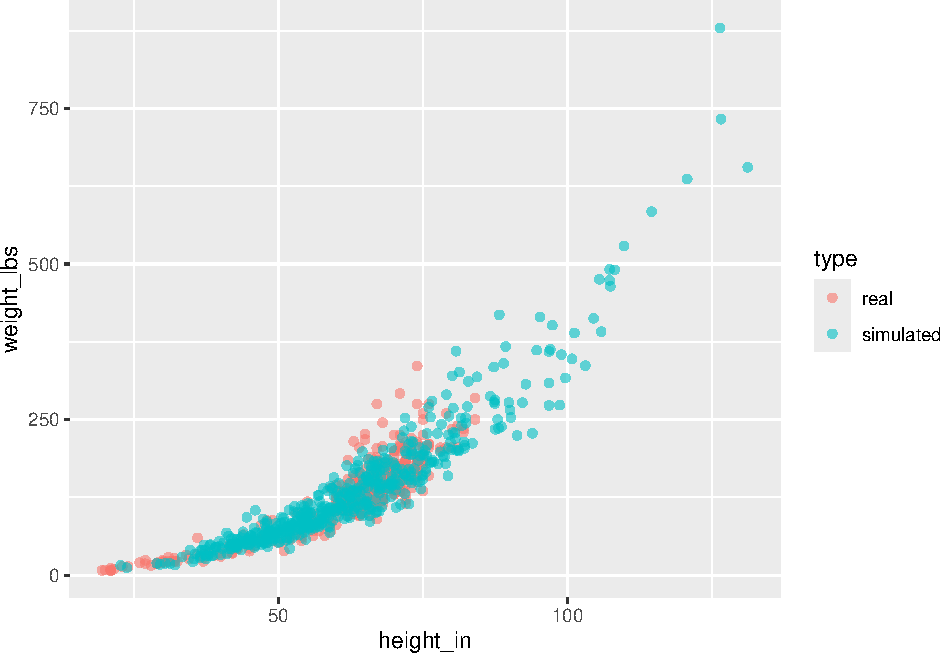
\includegraphics{L6_Correlation_and_regresion_simulation_pdf_files/figure-latex/plot sim data-1.pdf}

\hypertarget{with-tidyplots}{%
\section{\texorpdfstring{With
\textbf{\texttt{tidyplots}}}{With tidyplots}}\label{with-tidyplots}}

\begin{Shaded}
\begin{Highlighting}[]
\CommentTok{\# plot the data}
\NormalTok{all\_data }\SpecialCharTok{|\textgreater{}}
  \FunctionTok{tidyplot}\NormalTok{(}\AttributeTok{x =}\NormalTok{ height\_in, }
           \AttributeTok{y =}\NormalTok{ weight\_lbs,}
           \AttributeTok{color =}\NormalTok{ type) }\SpecialCharTok{|\textgreater{}}
  \FunctionTok{add\_data\_points}\NormalTok{(}\AttributeTok{alpha =}\NormalTok{ .}\DecValTok{6}\NormalTok{) }\SpecialCharTok{|\textgreater{}}
  \FunctionTok{adjust\_x\_axis\_title}\NormalTok{(}\StringTok{"Log of height in inches"}\NormalTok{) }\SpecialCharTok{|\textgreater{}}
  \FunctionTok{adjust\_y\_axis\_title}\NormalTok{(}\StringTok{"Log of weight in inches"}\NormalTok{)}
\end{Highlighting}
\end{Shaded}

\begin{center}\rule{0.5\linewidth}{0.5pt}\end{center}

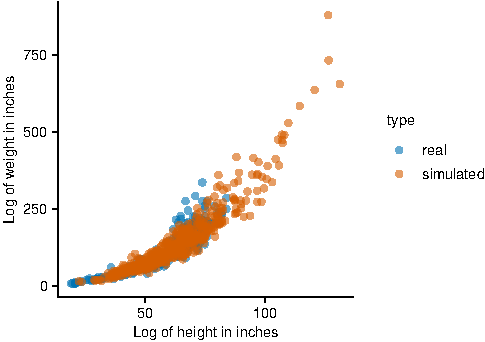
\includegraphics{L6_Correlation_and_regresion_simulation_pdf_files/figure-latex/tidyplot sim data 2-1.pdf}

\hypertarget{save-the-simulated-dataset}{%
\section{Save the simulated dataset}\label{save-the-simulated-dataset}}

\begin{Shaded}
\begin{Highlighting}[]
\CommentTok{\# write data as a csv into "data" folder}
\FunctionTok{write\_csv}\NormalTok{(all\_data, }\StringTok{"data\_tidy/simulated\_handw.csv"}\NormalTok{)}
\end{Highlighting}
\end{Shaded}

\hypertarget{round-up-and-conclusion}{%
\section{Round-up and conclusion}\label{round-up-and-conclusion}}

\begin{itemize}
\tightlist
\item
  In the process of showing you how to simulate bivariate data you
  become more familiar with covariance and matrix calculations.
\item
  This is just an example of how data simulation can develop statistical
  your expertise.
\item
  The end result is something you can use for research (e.g., your
  analysis script) or for teaching your class (e.g., the dataset).
\end{itemize}

\begin{center}\rule{0.5\linewidth}{0.5pt}\end{center}

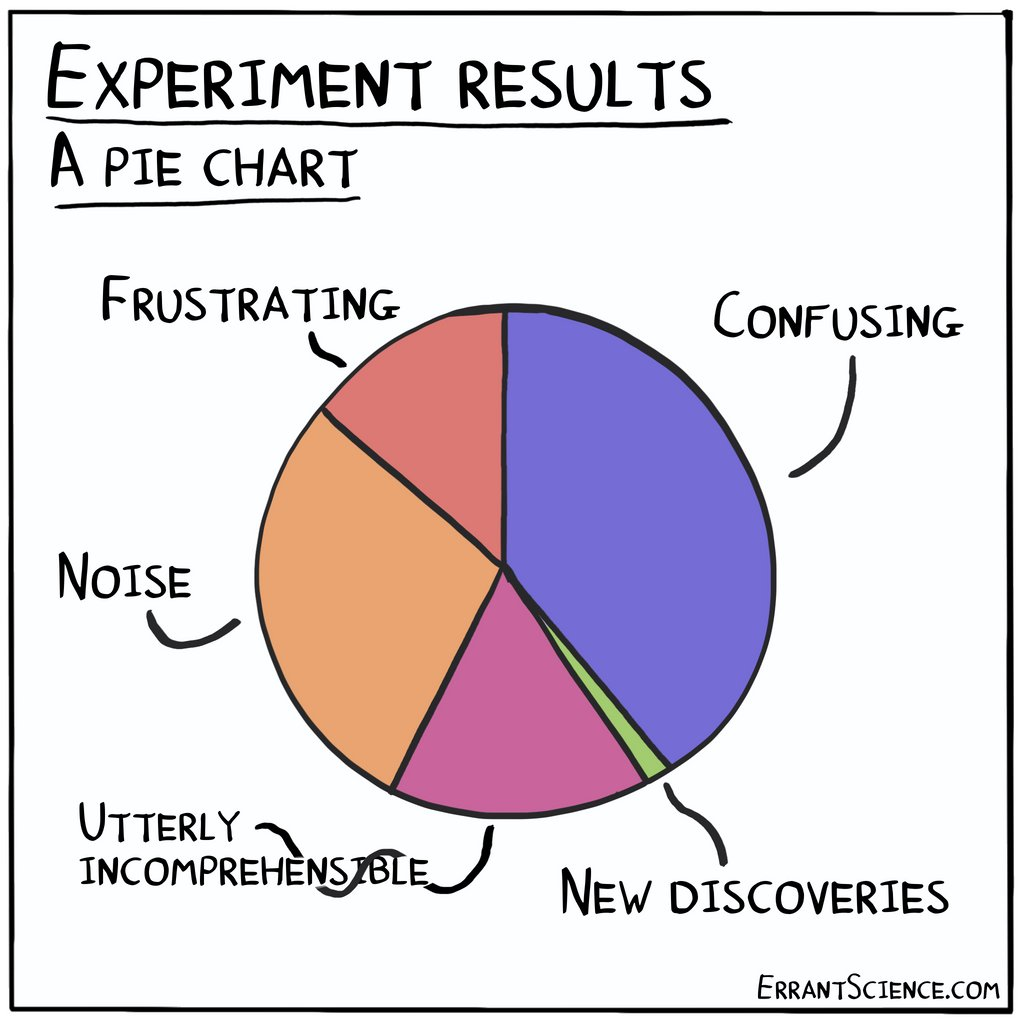
\includegraphics{images/experiment-results.jpg}

\hypertarget{thank-you}{%
\section{Thank you!}\label{thank-you}}

\emph{Inspiration for today's session on Data
Simulation:}\href{https://psyteachr.github.io/stat-models-v1/correlation-and-regression.html}{Learning
Statistical Models Through Simulation in R: Correlation and Regression}

\href{https://simsummerschool.github.io/}{PsyPag \& MSCP-Section
Simulation Summer School}

\href{https://debruine.github.io/data-sim-workshops/}{Data Simulation
Workshops}

\href{https://www.geogebra.org/m/RRprACv4}{Heights and weights dataset}

\end{document}
